\part{Research presentations}
\frame{\partpage}

\begin{frame}{Presentations}
    \begin{itemize}
        \pause\item Prepare and deliver a \textbf{brief presentation} on your research journal
        \pause\item Maximum \textbf{four minutes}, maximum \textbf{three slides}
        \pause\item Summarise the \textbf{context} in which your chosen paper is situated
        \pause\item Outline the \textbf{contributions} of your chosen paper to the field of computing
        \pause\item Describe the \textbf{influence} of your chosen paper on work that came since
    \end{itemize}
\end{frame}

\begin{frame}{Schedule}
    \begin{itemize}
        \pause\item Presentations are timetabled for \textbf{week 7}
        \pause\item \textbf{Running order} will be released \textbf{next week}
        \begin{itemize}
            \pause\item Half of you will present Monday, the other half Friday
        \end{itemize}
        \pause\item \textbf{All students} are expected to attend \textbf{the full duration of both sessions} to listen and support their peers
    \end{itemize}
\end{frame}

\begin{frame}{Paper selection --- please do ASAP!}
    \begin{center}
        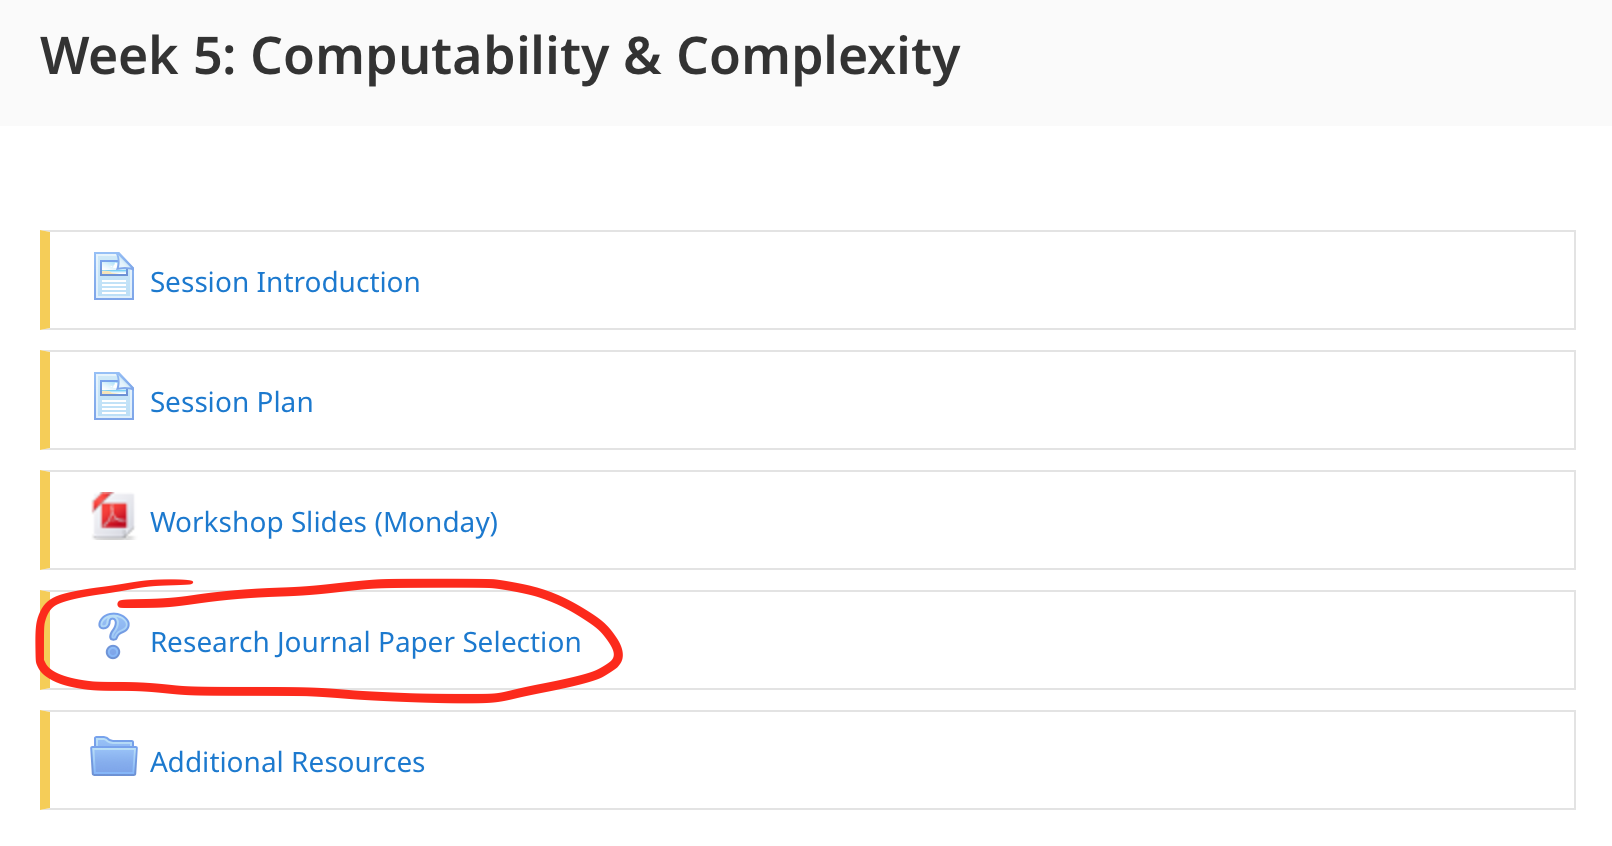
\includegraphics[width=0.9\textwidth]{paper_selection}
    \end{center}
\end{frame}

\begin{frame}{Slides}
    \begin{itemize}
        \pause\item Prepare your slides in \textbf{PowerPoint} or \textbf{PDF} format
        \begin{itemize}
            \pause\item If not using PowerPoint or Beamer, export your slides in one of these formats
            \pause\item Slides ``in the cloud'' are \textbf{not} acceptable!
        \end{itemize}
        \pause\item Upload your slides to LearningSpace by \textbf{11:59pm on Friday 1st November}
    \end{itemize}
\end{frame}

\begin{frame}{Slides upload}
    \begin{center}
        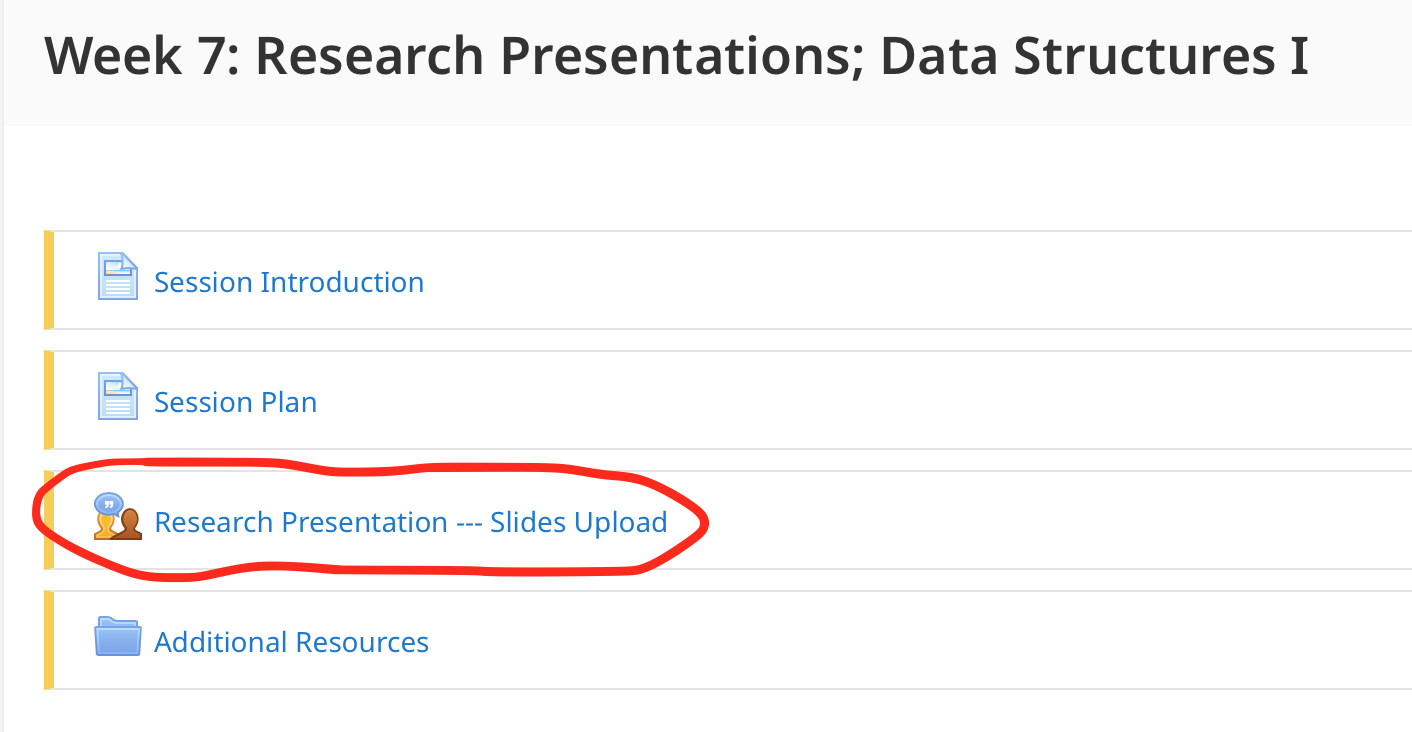
\includegraphics[width=0.9\textwidth]{slides_upload}
    \end{center}
\end{frame}

